For the case where the coronary artery has atherosclerosis, 
the problem is modeled as a flow between curved plates. 
The geometry used promotes a smooth reduction of the 
distance between the upper wall and symmetry axis of the channel. 
Due to atherosclerosis, 40\% channel obstruction was considered 
and the domain was discretized using 10261 nodes and 23049 
linear triangular elements. 

\par 
The \ref{velocity evolution curved} shows the unsteady velocity 
profile in the middle of the channel ($x=5R$). 
As we can see, the maximum non-dimensional value of the velocity field 
reaches $ u=2.3$ when the artery has atherosclerosis, that is, 
there is an increase of $53$\% of the maximum velocity when 
compared to the artery without atherosclerosis as shown in 
\ref{velocidade half poiseuille}.



\begin{figure}[H]
     \centering
     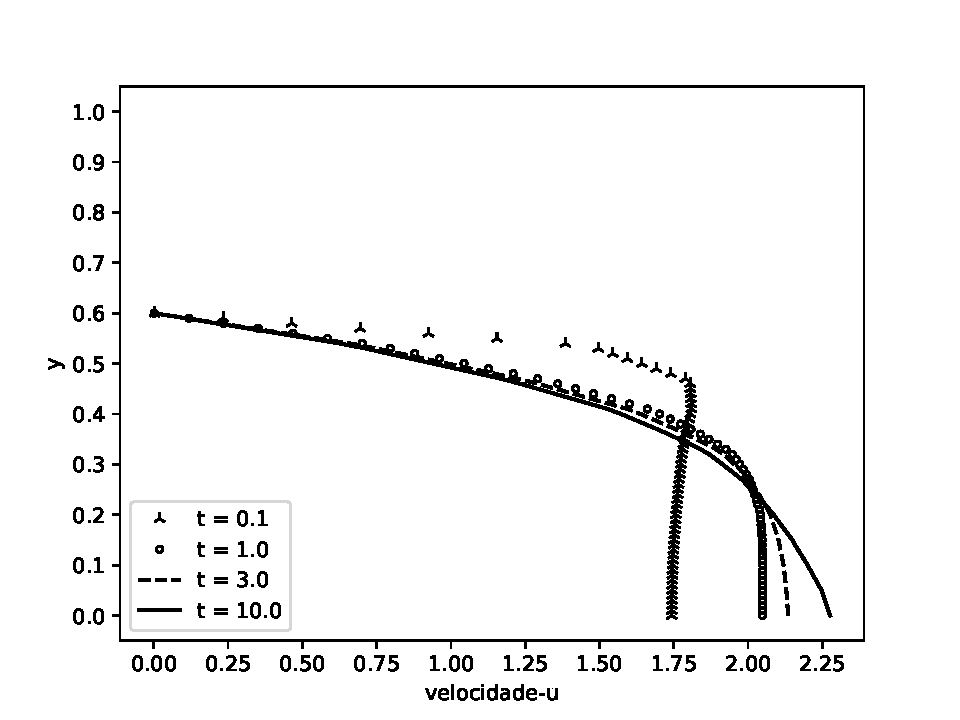
\includegraphics[scale=1]{./02_chaps/cap_solution/figure/vel_Curved_evol.pdf}\\
     \caption{The unsteady velocity profile for the curved channel.}
     \label{velocity evolution curved}
\end{figure}

\newpage
The \ref{velocity field curved} shows the evolution in time and space 
of the velocity field for half of the domain
The velocity field is represented with non-dimensional values 
where the red color refers to the value $u=2.3$ and 
the blue color $u=0$ approximately. Converting to dimensional values 
we have $u=27.6cm/s$ and $u=0cm/s$ respectively.

\vspace{2cm} 
\begin{figure}[H]
     \begin{minipage}{.50\linewidth}
      \centering
      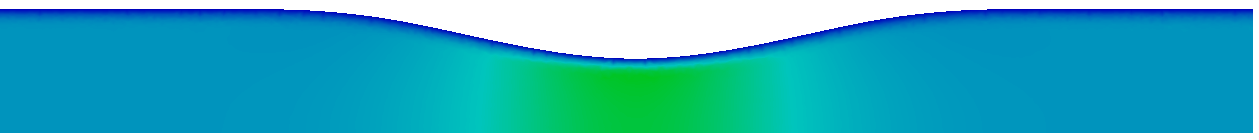
\includegraphics[scale=0.175]{./02_chaps/cap_solution/figure/vel_Curved200.png}\\
      t = 0.1
     \end{minipage}%
     \begin{minipage}{.50\linewidth}
      \centering
      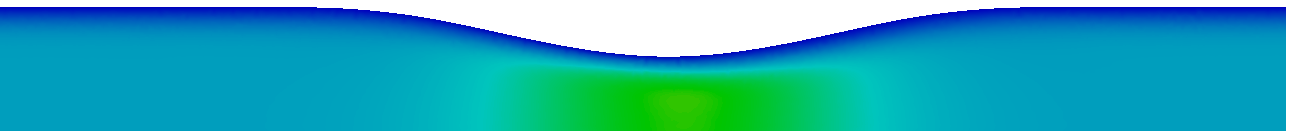
\includegraphics[scale=0.172]{./02_chaps/cap_solution/figure/vel_Curved1000.png}\\
      t = 0.5
     \end{minipage}
     \begin{minipage}{.50\linewidth}
     \medskip
      \centering
      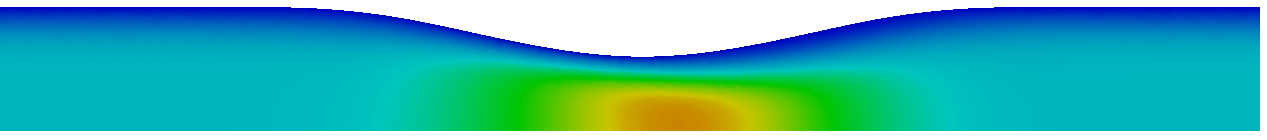
\includegraphics[scale=0.175]{./02_chaps/cap_solution/figure/vel_Curved2000.png}\\
      t = 1.0
     \end{minipage}%
     \begin{minipage}{.50\linewidth}
     \medskip
      \centering
      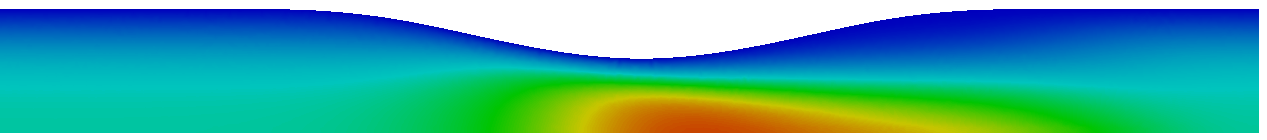
\includegraphics[scale=0.175]{./02_chaps/cap_solution/figure/vel_Curved6000.png}\\
      t = 3.0
     \end{minipage}
     \begin{minipage}{.50\linewidth}
      \centering
      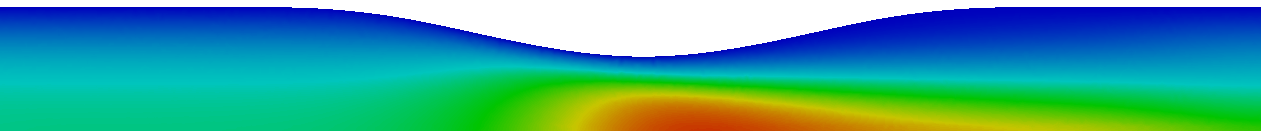
\includegraphics[scale=0.175]{./02_chaps/cap_solution/figure/vel_Curved8000.png}\\
      t = 4.0
     \end{minipage}%
     \begin{minipage}{.50\linewidth}
      \centering
      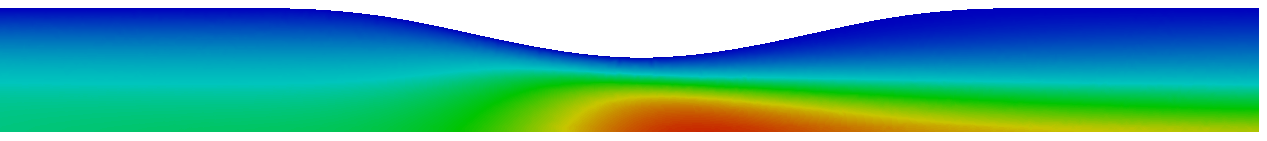
\includegraphics[scale=0.175]{./02_chaps/cap_solution/figure/vel_Curved10000.png}\\
      t = 5.0
     \end{minipage}
     \begin{minipage}{.50\linewidth}
     \medskip
      \centering
      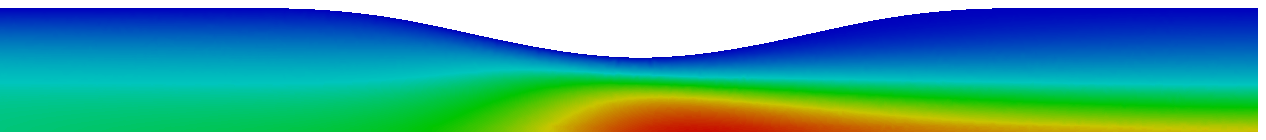
\includegraphics[scale=0.175]{./02_chaps/cap_solution/figure/vel_Curved14000.png}\\
      t = 7.0
     \end{minipage}%
     \begin{minipage}{.50\linewidth}
     \medskip
      \centering
      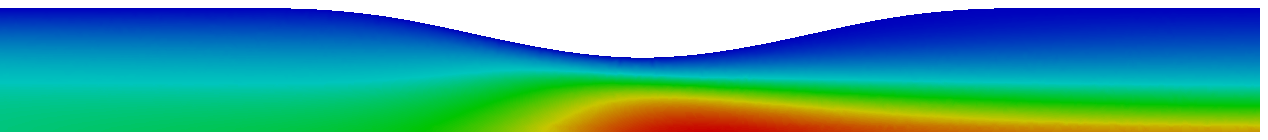
\includegraphics[scale=0.175]{./02_chaps/cap_solution/figure/vel_Curved20000.png}\\
      t = 10.0
     \end{minipage}
     \medskip
     \caption{Time and space evolution of the velocity field for curved channel.}
     \label{velocity field curved}
\end{figure}

